\begin{enumerate}
\item En primer lugar se diseñan 4 filtros elípticos usando el comando \texttt{ellip} de MATLAB. Las especificacones de dichos filtros son:
\begin{itemize}
    \item Filtro a: Pasa bajos orden 2 ($f_c = 2 kHz$).
    \item Filtro b: Pasa altos orden 2 ($f_c = 4 kHz$)
    \item Filtro c: Pasa banda orden 4 ($f_1 = 2 kHz, f_2 = 4 kHz$)
    \item Filtro d: Elimina banda orden 4 ($f_1 = 2 kHz, f_2 = 4 kHz$)
\end{itemize}
como suposición se escogió:
\begin{itemize}
    \item Ripple en banda de paso: 5 dB.
    \item Atenuación en banda de rechazo: 20 dB.
\end{itemize}

La sintaxis típica del comando \texttt{ellip} es: \texttt{[b,a] = ellip(n,Rp, Rs, Wn, Ftype)} donde:
\begin{itemize}
    \item \texttt{b}: Coeficientes de la parte MA del filtro.
    \item \texttt{a}: Coeficientes de la parte AR del filtro.
    \item \texttt{n}: Orden del filtro
    \item \texttt{Rp}: Ripple máximo tolerado en banda de paso.
    \item \texttt{Rs}: Atenuación en banda de rechazo
    \item \texttt{Wn}: Frecuencia o frecuencias de corte en $\pi\cdot$rad/muestra
    \item \texttt{Ftype}: Tipo de filtro (pasa bajos, pasa altos, pasabanda o elimina banda).
\end{itemize}

Con las suposiciones tomadas y las condiciones del diseño del filtro se diseñan los filtros usando el siguiente segmento de código:
\begin{lstlisting}[frame=single]
%%% 1. Diseno de filtros IIR usando ellip

%ordenes
n1a = 2; n1b = 2; n1c = 4; n1d = 4;
%frecuencias de corte normalizadas (pasa bajos y pasa altos)
Fs = 16000; fc1_a1_Hz = 2000; fc1_a1 = fc1_a1_Hz/Fs;%filtro a
fc1_b1_Hz = 4000; fc1_b1 = fc1_b1_Hz/Fs;            %filtro b
%frecuencias normalizadas (pasa banda y elimina banda)
f1_c1_Hz = 2000; f1_c1 = f1_c1_Hz/Fs;               %filtro c
f1_c2_Hz = 4000; f1_c2 = f1_c2_Hz/Fs;
f1_d1_Hz = 2000; f1_d1 = f1_d1_Hz/Fs;               %filtro d
f1_d2_Hz = 4000; f1_d2 = f1_d2_Hz/Fs;
%Suposiciones de ripple y banda de rechazo
Rp = 5; Rs = 20; %Ripple banda de paso y atenuacion (rechazo)  
%Diseno de Filtros 
[b1_a, a1_a]=ellip(n1a, Rp, Rs, 2*fc1_a1, "low");
[b1_b, a1_b]=ellip(n1b, Rp, Rs, 2*fc1_b1, "high");
[b1_c, a1_c]=ellip(n1c, Rp, Rs, 2*[f1_c1 f1_c2], "bandpass");
[b1_d, a1_d]=ellip(n1d, Rp, Rs, 2*[f1_d1 f1_d2], "stop");
\end{lstlisting}

Las respuestas en frecuencia de los filtros diseñados se muestran en las figuras \ref{fig:p4_1a}, \ref{fig:p4_1b}, \ref{fig:p4_1c} y \ref{fig:p4_1d}. Se aprecia que se cumplen los requisitos de diseño.
\begin{figure}[H]
    \centering
    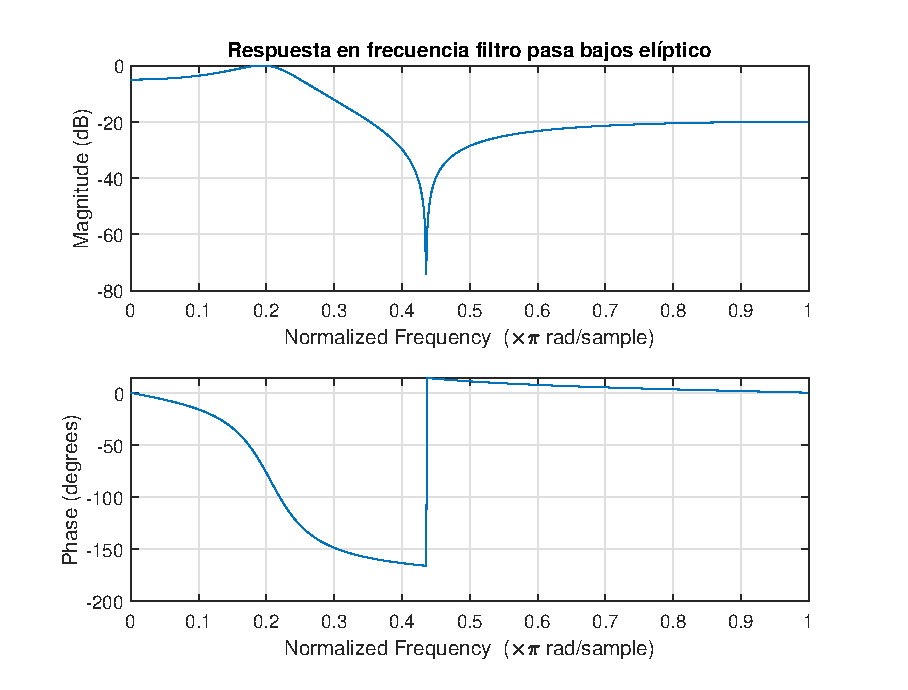
\includegraphics[width = .8\linewidth]{Figuras/p4_1a.eps}
    \caption{Respuesta en frecuencia de filtro pasa bajos diseñado usando \texttt{ellip}, de orden 2, $f_c = 2 kHz$, ripple en banda de paso 5 dB y atenuación de 20 dB en banda de rechazo.}
    \label{fig:p4_1a}
\end{figure}

\begin{figure}[H]
    \centering
    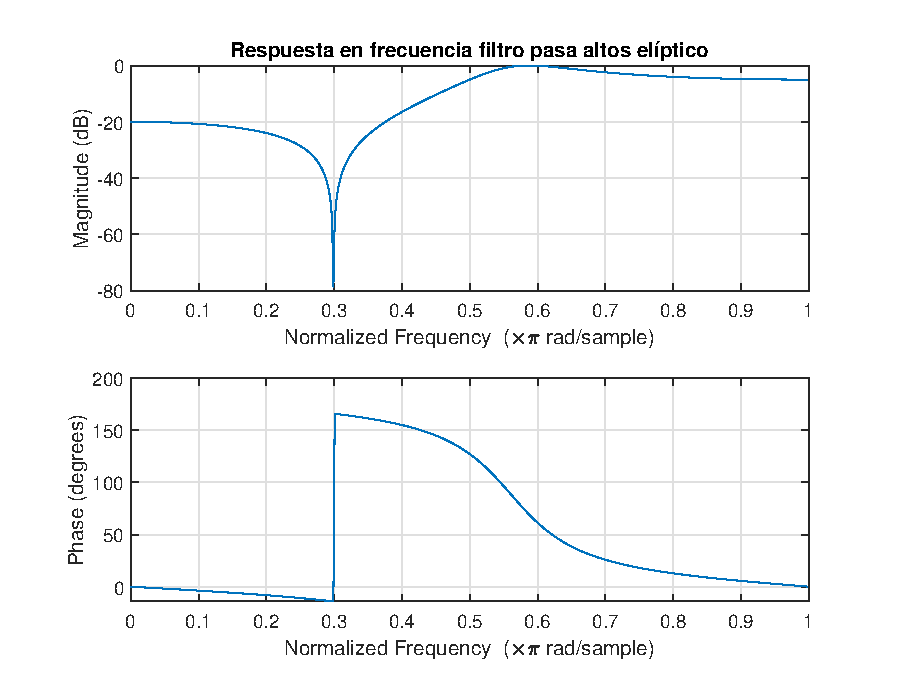
\includegraphics[width = .8\linewidth]{Figuras/p4_1b.eps}
    \caption{Respuesta en frecuencia de filtro pasa altos diseñado usando \texttt{ellip}, de orden 2, $f_c = 4 kHz$, ripple en banda de paso de 5 dB y atenuación de 20 dB en banda de rechazo.}
    \label{fig:p4_1b}
\end{figure}

\begin{figure}[H]
    \centering
    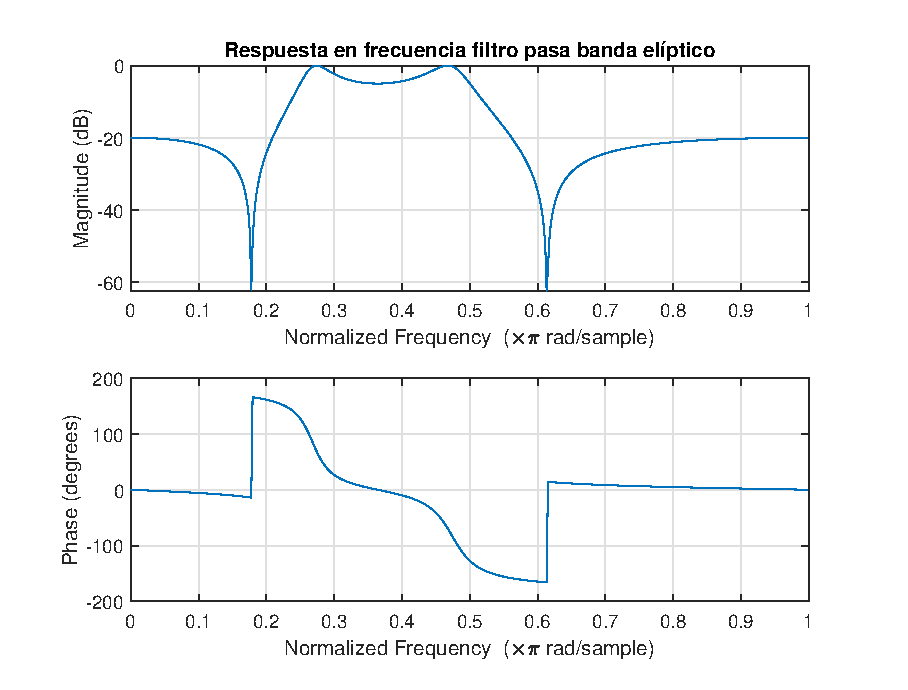
\includegraphics[width = .8\linewidth]{Figuras/p4_1c.eps}
    \caption{Respuesta en frecuencia de filtro pasa banda diseñado usando \texttt{ellip}, de orden 4, $f_1 = 2 kHz, f_2= 4 kHz$, ripple en banda de paso de 5 dB y atenuación de 20 dB en banda de rechazo.}
    \label{fig:p4_1c}
\end{figure}

\begin{figure}[H]
    \centering
    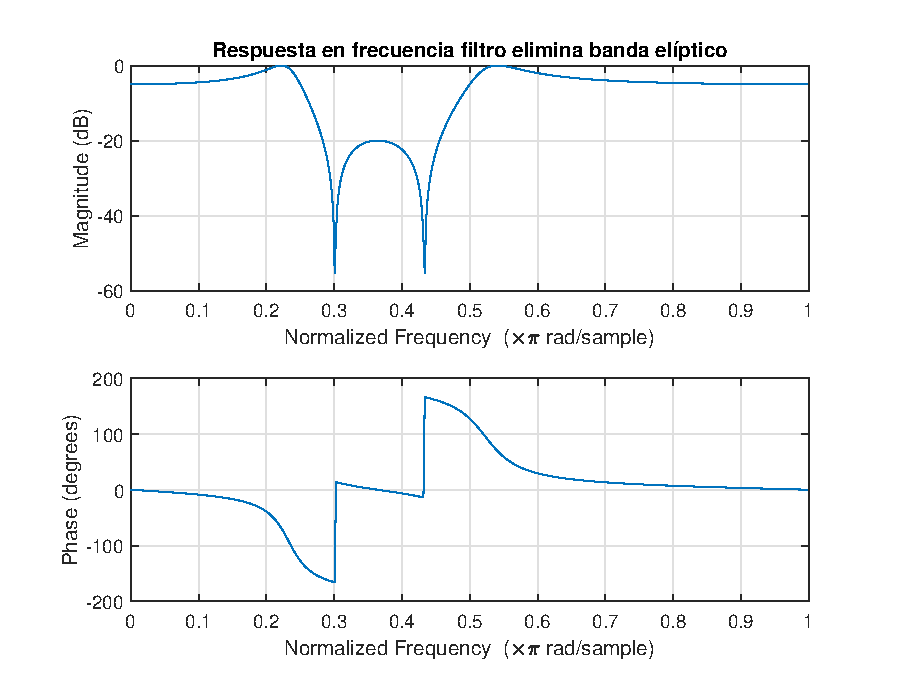
\includegraphics[width = .8\linewidth]{Figuras/p4_1d.eps}
    \caption{Respuesta en frecuencia de filtro elimina banda diseñado usando \texttt{ellip}, de orden 4, $f_1 = 2 kHz, f_2= 4 kHz$, ripple en banda de paso de 5 dB y atenuación de 20 dB en banda de rechazo.}
    \label{fig:p4_1d}
\end{figure}

\item Se pide diseñar 2 filtros pasabanda usando los comandos de MATLAB \texttt{cheby1} y \texttt{cheby2}, considerando frecuencias de corte $f_1 = 2$ kHz y $f_2 = 4$  kHz, una frecuencia de muestreo de 16 kHz y orden 4.

Para un filtro se pide 2 dB máximo de ripple en la banda de paso y para el otro 20 dB de atenuación en la banda de rechazo. Debido a que el filtro de chebishev tipo I es un filtro que permite una región de transición corta dado un máximo de ripple en la banda de paso se uso \texttt{cheby1} para el primer filtro. Para el segundo se usó \texttt{cheby2} pues el filtro de chebishev tipo II  permite asegurar un mínimo de atenuación.

La sección de código para el diseño de los filtros se muestra a continuación

\begin{lstlisting}[frame=single]
%% 2. Diseno de filtros chebyshev tipo I y II

%orden
n2 = 4;
%frecuencias de corte
f2_1_Hz = 2000; f2_1 = f2_1_Hz/Fs;
f2_2_Hz = 4000; f2_2 = f2_2_Hz/Fs;
%Restricciones de Ripple
Rp = 2; Rs = 20;
%Diseno de Filtros [b,a] = cheby1(n,Rp,Wp,ftype)
[b2_a, a2_a] = cheby1(n2, Rp, 2*[f2_1 f2_2], "bandpass");
[b2_b, a2_b] = cheby2(n2, Rs, 2*[f2_1 f2_2], "bandpass");
\end{lstlisting}

Las imágenes de respuesta en frecuencia para el filtro a y b diseñados se muestran en las figuras \ref{} y \ref{} respectivamente. Se aprecia que se cumplen los requisitos de diseño.

\begin{figure}[H]
    \centering
    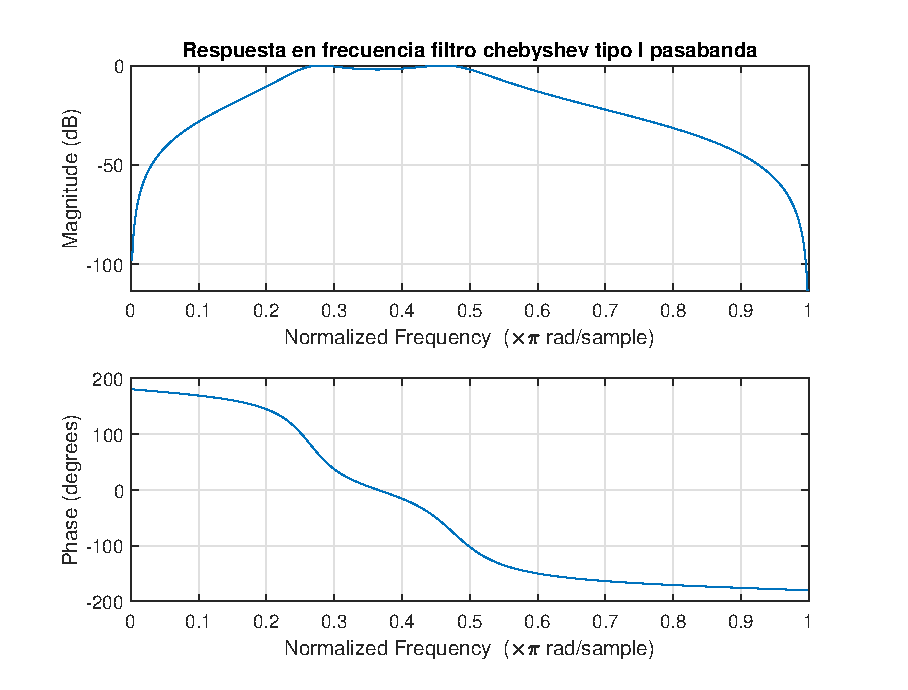
\includegraphics[width = .8\linewidth]{Figuras/p4_2a.eps}
    \caption{Respuesta en frecuencia de filtro pasa banda con ripple máximo de 2 dB en banda de paso, diseñado usando estructura de filtro chebyshev tipo I.}
    \label{fig:p4_2a}
\end{figure}

\begin{figure}[H]
    \centering
    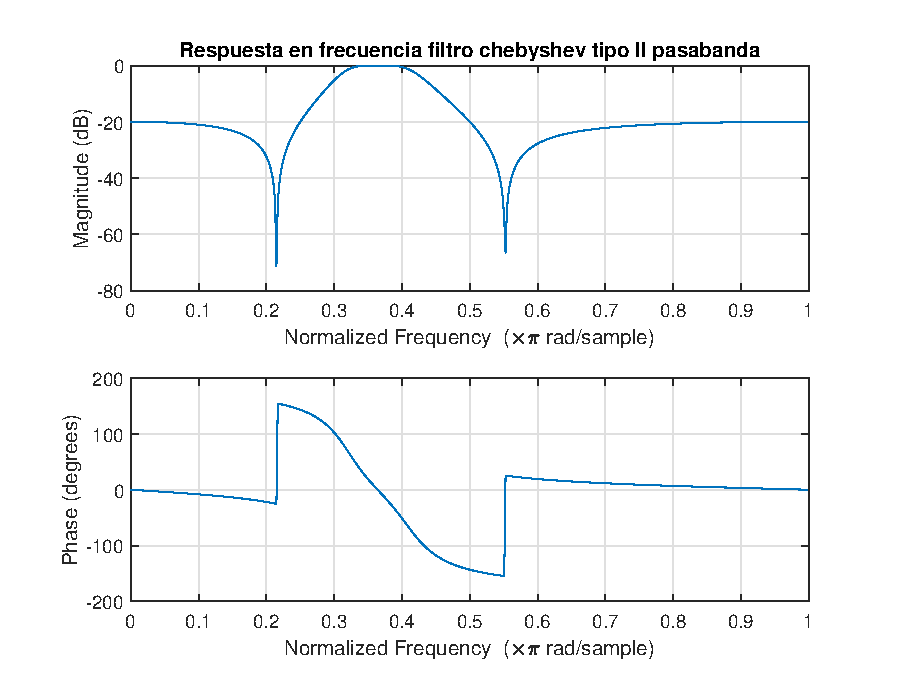
\includegraphics[width = .8\linewidth]{Figuras/p4_2b.eps}
    \caption{Respuesta en frecuencia de filtro pasa banda con atenuación mínima de 20 dB en banda de rechazo, diseñado usando estructura de filtro chebyshev tipo II.}
    \label{fig:p4_2b}
\end{figure}

De evaluar la respuesta en frecuencia del filtro chebyshev tipo I diseñado se obtiene que:
\begin{align*}
    h_{I}(f_1 = 2000 \text{ Hz}) &= h_{I}\left(0.25  \dfrac{\pi\text{rad}}{\text{sample}}\right) \approx -32.76 \text{ dB} \\
    h_{I}(f_1 = 4000 \text{ Hz}) &= h_{I}\left(0.5  \dfrac{\pi\text{rad}}{\text{sample}}\right) \approx -17.81 \text{ dB} \\
\end{align*}

De evaluar la respuesta en frecuencia del filtro chebyshev tipo II diseñado se obtiene que:
\begin{align*}
    h_{II}(f_1 = 2000 \text{ Hz}) &= h_{II}\left(0.25  \dfrac{\pi\text{rad}}{\text{sample}}\right) \approx -20.61 \text{ dB} \\
    h_{II}(f_1 = 4000 \text{ Hz}) &= h_{II}\left(0.5  \dfrac{\pi\text{rad}}{\text{sample}}\right) \approx -23.87 \text{ dB} \\
\end{align*}

\item Se pide diseñar un filtro butterworth pasa banda de orden 4, con frecuencias de corte $f_1 = 800$ Hz y $f_2 = 1600$ Hz usando el comando \texttt{butter}, considerando una frecuencia de muestreo de 16 kHz. La sección de código se muestra a continuación:
\newpage
\begin{lstlisting}[frame=single]
%%% 3. Diseno de filtros butterworth

%orden
n3 = 4/2;
%frecuencias de corte
f3_1_Hz = 800 ; f3_1 = f3_1_Hz/Fs;
f3_2_Hz = 1600; f3_2 = f3_2_Hz/Fs;
%Diseño de Filtros
[b3, a3] = butter(n3, 2*[f3_1 f3_2], "bandpass");
\end{lstlisting}

La respuesta en frecuencia del filtro diseñado se muestra en la figura \ref{fig:p4_3}.

\begin{figure}[H]
    \centering
    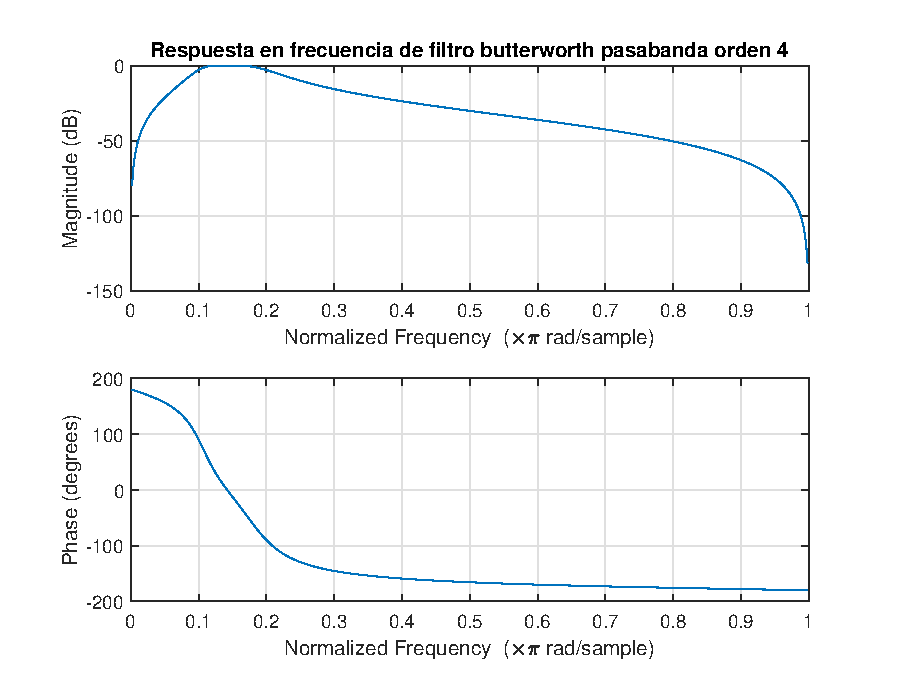
\includegraphics[width = .8\linewidth]{Figuras/p4_3.eps}
    \caption{Respuesta en frecuencia de filtro butterworth pasa banda de orden 4 diseñado.}
    \label{fig:p4_3}
\end{figure}

Posteriormente se hace un análisis de que ocurre con la ubicación de polos y ceros al diseñar filtros butterworth a medida que se aumenta el orden. La sección de código para aquello se muestra a continuación:
\begin{lstlisting}
%Analisis de polos y ceros butterworth 
n = [4 6 8 10 12 14];
figure
for i = 1:6
    [z,p,~] = butter(n(i)/2, 2*[f3_1 f3_2], "bandpass");
    subplot(3,2,i); zplane(z,p);
    title({"Diagrama de polos y ceros para filtro ", strcat(
        "butterworth pasabandas de orden ", int2str(n(i)))})
end
\end{lstlisting}

Los diagramas de polos y ceros se muestran en la figura \ref{fig:p4_3zp}. Notar que a medida que aumenta el orden del filtro los polos dominantes se acercan más al círculo unitario. Lo anterior podría volver el sistema inestable por temas numéricos.

\begin{figure}[H]
    \centering
    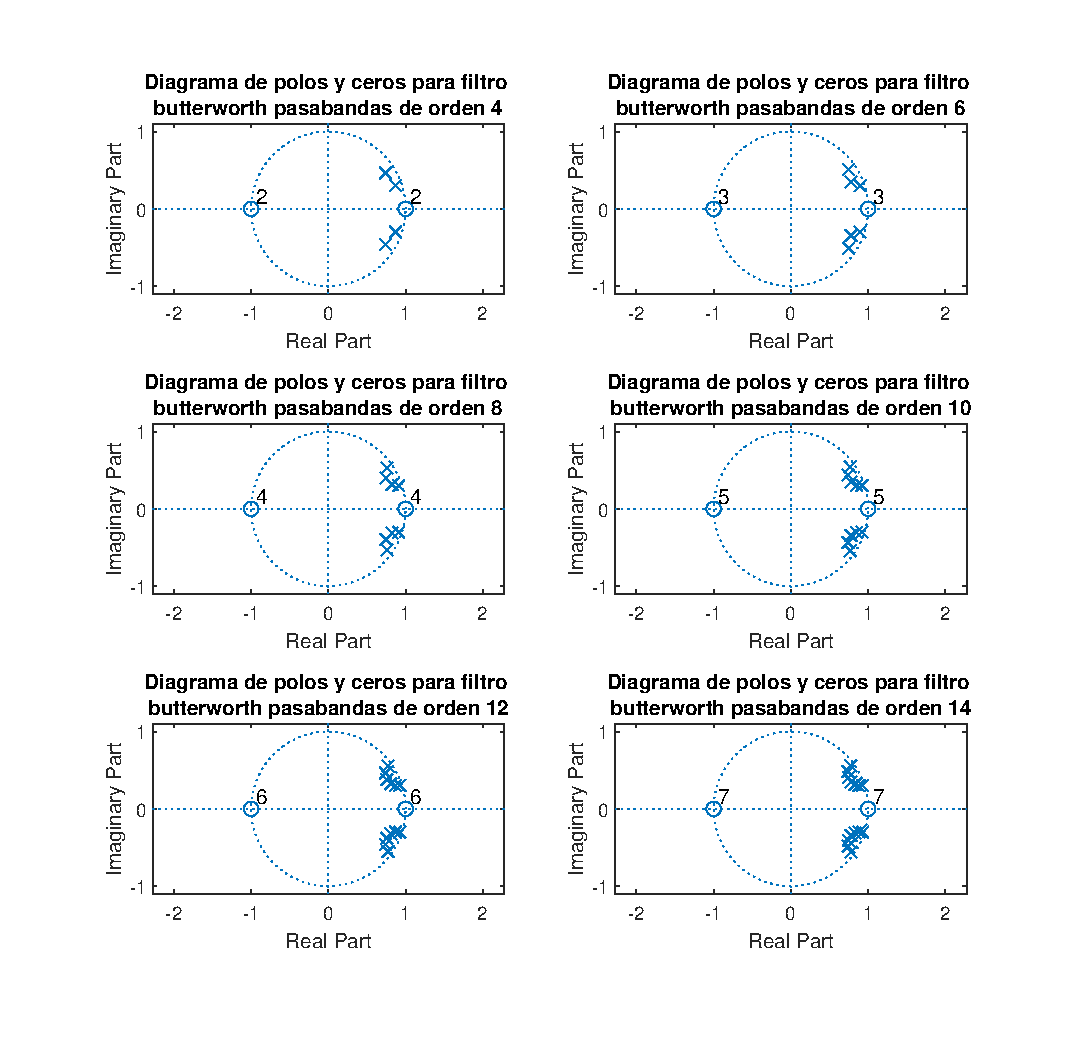
\includegraphics[width = .95\linewidth]{Figuras/p4_3_zp.eps}
    \caption{Diagramas de polos y ceros de filtros butterworth pasa banda de orden 4, 6, 8, 10, 12 y 14.}
    \label{fig:p4_3zp}
\end{figure}

\end{enumerate}